
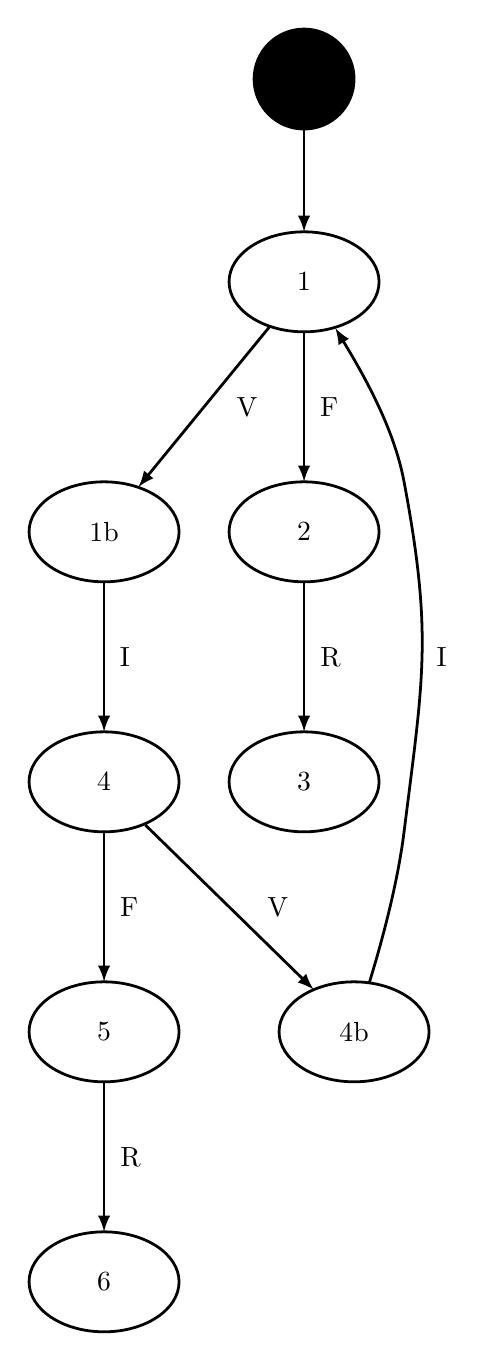
\begin{tikzpicture}[>=latex,line join=bevel,]
  \pgfsetlinewidth{1bp}
%%
\pgfsetcolor{black}
  % Edge: 2 -> 3
  \draw [->] (99bp,269.61bp) .. controls (99bp,257.24bp) and (99bp,240.37bp)  .. (99bp,216.05bp);
  \definecolor{strokecol}{rgb}{0.0,0.0,0.0};
  \pgfsetstrokecolor{strokecol}
  \draw (108.5bp,243bp) node {R};
  % Edge: 4b -> 1
  \draw [->] (122.49bp,125.7bp) .. controls (126.86bp,139.95bp) and (132.64bp,161.07bp)  .. (135bp,180bp) .. controls (141.93bp,235.57bp) and (145.33bp,250.96bp)  .. (135bp,306bp) .. controls (131.9bp,322.5bp) and (123.64bp,339.34bp)  .. (110.26bp,361.32bp);
  \draw (148.5bp,243bp) node {I};
  % Edge: 5 -> 6
  \draw [->] (27bp,89.614bp) .. controls (27bp,77.24bp) and (27bp,60.369bp)  .. (27bp,36.05bp);
  \draw (36.5bp,63bp) node {R};
  % Edge: 4 -> 4b
  \draw [->] (41.862bp,182.47bp) .. controls (56.278bp,168.37bp) and (78.332bp,146.81bp)  .. (102.41bp,123.26bp);
  \draw (89.5bp,153bp) node {V};
  % Edge: 4 -> 5
  \draw [->] (27bp,179.61bp) .. controls (27bp,167.24bp) and (27bp,150.37bp)  .. (27bp,126.05bp);
  \draw (36bp,153bp) node {F};
  % Edge: 1 -> 2
  \draw [->] (99bp,359.61bp) .. controls (99bp,347.24bp) and (99bp,330.37bp)  .. (99bp,306.05bp);
  \draw (108bp,333bp) node {F};
  % Edge: 0 -> 1
  \draw [->] (99bp,432.81bp) .. controls (99bp,424.79bp) and (99bp,415.05bp)  .. (99bp,396.03bp);
  % Edge: 1 -> 1b
  \draw [->] (86.459bp,361.67bp) .. controls (75.308bp,348.04bp) and (58.84bp,327.92bp)  .. (39.398bp,304.15bp);
  \draw (78.5bp,333bp) node {V};
  % Edge: 1b -> 4
  \draw [->] (27bp,269.61bp) .. controls (27bp,257.24bp) and (27bp,240.37bp)  .. (27bp,216.05bp);
  \draw (34.5bp,243bp) node {I};
  % Node: 1
\begin{scope}
  \definecolor{strokecol}{rgb}{0.0,0.0,0.0};
  \pgfsetstrokecolor{strokecol}
  \draw (99bp,378bp) ellipse (27bp and 18bp);
  \draw (99bp,378bp) node {1};
\end{scope}
  % Node: 0
\begin{scope}
  \definecolor{strokecol}{rgb}{0.0,0.0,0.0};
  \pgfsetstrokecolor{strokecol}
  \definecolor{fillcol}{rgb}{0.0,0.0,0.0};
  \pgfsetfillcolor{fillcol}
  \filldraw [opacity=1] (99bp,451bp) ellipse (18bp and 18bp);
\end{scope}
  % Node: 3
\begin{scope}
  \definecolor{strokecol}{rgb}{0.0,0.0,0.0};
  \pgfsetstrokecolor{strokecol}
  \draw (99bp,198bp) ellipse (27bp and 18bp);
  \draw (99bp,198bp) node {3};
\end{scope}
  % Node: 2
\begin{scope}
  \definecolor{strokecol}{rgb}{0.0,0.0,0.0};
  \pgfsetstrokecolor{strokecol}
  \draw (99bp,288bp) ellipse (27bp and 18bp);
  \draw (99bp,288bp) node {2};
\end{scope}
  % Node: 5
\begin{scope}
  \definecolor{strokecol}{rgb}{0.0,0.0,0.0};
  \pgfsetstrokecolor{strokecol}
  \draw (27bp,108bp) ellipse (27bp and 18bp);
  \draw (27bp,108bp) node {5};
\end{scope}
  % Node: 4
\begin{scope}
  \definecolor{strokecol}{rgb}{0.0,0.0,0.0};
  \pgfsetstrokecolor{strokecol}
  \draw (27bp,198bp) ellipse (27bp and 18bp);
  \draw (27bp,198bp) node {4};
\end{scope}
  % Node: 6
\begin{scope}
  \definecolor{strokecol}{rgb}{0.0,0.0,0.0};
  \pgfsetstrokecolor{strokecol}
  \draw (27bp,18bp) ellipse (27bp and 18bp);
  \draw (27bp,18bp) node {6};
\end{scope}
  % Node: 1b
\begin{scope}
  \definecolor{strokecol}{rgb}{0.0,0.0,0.0};
  \pgfsetstrokecolor{strokecol}
  \draw (27bp,288bp) ellipse (27bp and 18bp);
  \draw (27bp,288bp) node {1b};
\end{scope}
  % Node: 4b
\begin{scope}
  \definecolor{strokecol}{rgb}{0.0,0.0,0.0};
  \pgfsetstrokecolor{strokecol}
  \draw (117bp,108bp) ellipse (27bp and 18bp);
  \draw (117bp,108bp) node {4b};
\end{scope}
%
\end{tikzpicture}

